% The setting of the project is described based on the scientific literature in a balanced and comprehensive way. The content and relevance of the included literature is understood
\chapter[Background]{Background}
\label{cha:backgr}
This chapter will go over the background of this project, which will cover basic operating system fundamentals, a brief overview of the RISC-V architecture, and the specifics of the board that will be used, which is the Sifive Hifive1 RevB. By the end of the chapter, the reader should be able to understand how parts of the operating system should function, and be able to understand the RISC-V architecture in comparison to the ARM architecture.
\section{Operating System Fundamentals}
An operating system's purpose is to provide an interface between user code and the hardware, such as memory and \ac{io}, to allow the user code to function seamlessly, and allow interaction with users. This has been split into three key sections, as listed by the aims of the project, as process management, memory management and \ac{io} management\cite{modern_operating}.
\subsection{Process Management}
A process is a section of executing code along with the registers that executing code uses. The goal of the operating system is to allow multiple processes to run at once. In a system with multiple hardware threads, this would be possible to do explicitly, as the different threads could simply execute the processes. However the desired number of processes is almost always higher than the number of available threads, and in the world of microprocessors there is rarely more than one thread, so instead processes must be run individually and interleaved to give the illusion of multitasking, provided that this is done at a high enough frequency. There are several methods and approaches to this task\cite{modern_operating}.
\subsubsection{Scheduling Algorithms}
The main approaches to be considered for scheduling algorithms for this project will be a batch approach and an interactive approach. The most important distinction between the two is the inclusion of preemption. In a batch system, a non-preemptive approach will be taken, where once a processes execution is began, it will be allowed to be completed before any other process is ran. This creates a simple system and is used is situations where completion of tasks is not expected to be quick. The main challenges of this approach is in process execution time estimation, as this allows the scheduler to order the execution of processes in a way that ensure small tasks are allowed to run. In an interactive system, it is expected from the user that interactions should have quick responses. This introduces the need for preemption, where a processes' execution may be paused after a short period of time to allow other processes to be ran. By running each process in small interleaved sections this allows multiple processes functionally at the same time, which means processes from which a user is expecting a response will not get halted by a larger process\cite{modern_operating}.
\subsection{Memory Management}
The goal of memory management is to streamline how a process can use memory, while at the same time protecting critical sections of memory from faulty or malicious user code. In a system with multiple processes being executed and no memory abstraction, there exists the possibility that two processes attempt to use the same section of memory, creating a conflict that would cause both processes to run incorrectly. This occurs as different processes cannot be aware of each other, and have no choice but to use memory without knowledge of which sections are in use. This can be solved using memory abstraction. The simplest method of this is using address spaces, where each process is given permission to access only segments of directly addressed memory. This prevents each process modifying other processes memory, and allows the process to behave individually, as long as it is provided with the location of its address space\cite{modern_operating}.
\subsection{IO Management}
The device that the project features will have severely limited \ac{io}. For the purpose of this project there will be two categories of \ac{io}, programmed \ac{io} and interrupt driven \ac{io}. 
\subsubsection{Programmable \ac{io}}
Programmable \ac{io} is where actions that require \ac{io} are done in sequence, which will generally function by the user code making an environment call, which will then perform the \ac{io} operation, and return control to the user code once the operation is complete. This is not always desirable, as the operations are often slow and would require polling, which is the process of performing busy operations until a resource is free. During this time all processes are effectively blocked as the the environment call is not being preempted, so this process can significantly slow execution if large amounts of data is needed to be transferred. However this type of \ac{io} can be useful in cases where only small amounts of data is being transferred, for instance in cases where only single bytes are transferred the overhead needed for interrupt driven \ac{io} would be larger than the time lost to polling.
\subsubsection{Interrupt driven \ac{io}}
To avoid the blocking caused by polling, \ac{io} can be interacted with through the use of interrupts. This would be done by a process making an environment call similar to programmable \ac{io}, however in this case only the caller process would be blocked until the \ac{io} operation was complete. It would also enable some form of interrupt, which signals when the \ac{io} function is available to be used. At that point an interrupt will be raised and part of the operation with be completed until the \ac{io} is busy again, at which point execution is returned to all the unblocked processes. This means that there is no time wasted polling, although does introduce overhead in the form of interrupt calls, which if done too often could slow down execution to a similar level as polling.
\section{RISC-V}
RISC-V is \ac{risc} \ac{isa}, built with the goal to be completely open. The ISA uses a base integer ISA which can be used on its own or with a number of optional standard extensions, which is part of a goal to avoid `over-architecting' for particular micro-architectures. There are variants for both 32 bit systems and 64 bit systems however for this project only the 32 bit system will be considered\cite{riscv_unpriv}.
\subsection{Registers}
RISC-V implements 32 general purpose registers, which in our case will be 32 bits wide, and labeled x0 to x31. The x0 register is hardwired to zero, and all other registers may be used. There are no specific registers used for storing information like the stack pointer or return address, however in this project the standard calling convention will be used. This specifies how each register should be used, how the register should be saved, and gives each register a pseudonym which correlates to its purpose. Important registers are ra, which is used to store the return address produced by the jump and link instruction, sp and gp, which are used to store the stack pointer and the global pointer. The stack pointer is used to store the most recent item in the current processes stack, and the global pointer is used to point to the address space where a processes global variables will be stored. The collection of registers a0-a7 are used to pass arguments to functions, as well as a0 serving as a return value. For general use there are registers t0 to t6 and s0 to s11, the difference being that t0-t6 are temporary registers that are not required to have their value saved before use, whereas s0-s11 does require saving the value. This allows the use of temporary registers to store intermediate values or value not needed to be stored, without needed the overhead of adding them to the stack, and the saved registers allow important information not to be overwritten by called functions\cite{riscv_unpriv}.
\subsection{Base ISA}
The base ISA, known as RV32I, specifies the set of instructions that all RISC-V systems implement, which includes both privileged and unprivileged instructions. The load and store operations allow loading and storing one register to or from memory. This registers can be treated as a word, half word or as a byte. There are the standard arithmetic, logic and shift operations, however immediate values are limited to 12 bits, so operations such as LUI (load upper immediate) may be used to load larger immediate values into a register.\\
Unlike ARM, the RISC-V ISA does not use flags to determine conditional operations. Instead the condition that is used to determine whether a branch is taken or not is included in the branch operation itself, with instructions like BEQ (branch if equal) or BGT (branch if greater than). These are accompanied by comparison operations, which evaluate similar conditions, and produce either a 1 or a 0 in the target register. JAL (jump and link) branches to a specified location while storing a return address, which allows the implementation of subroutines and functions\cite{riscv_unpriv}.
\subsubsection{Privilege levels}
The previously described operations can be performed in any privilege mode. RISC-V can support up to three privilege modes, being user, supervisor, and machine mode, although this report will only be considering user mode and machine mode. The zicsr extension adds operations that allow a hart in machine mode to read and modify \ac{csrs}, such as the CSRRW, which reads a csr to a register and writes a register to a csr, although either the source or target register can be set to zero to disable either the reading or the writing. Also included is the CSRRS and CSRRC, which is similar to CSRRW but sets or clears bits of the \ac{csrs}. Machine mode also has full access to the full memory space, whereas a thread in user mode can only access memory that has been specified by the \ac{pmp}, producing an access fault otherwise\cite{riscv_unpriv}\cite{riscv_priv}.
\subsubsection{Optional Extensions}
% Include info on A, M, and C
There are several optional extensions that can be implemented. This includes the `C' extensions, which includes a reduced number of instructions from the base ISA, but in a 16 bit compressed format. The `M' extension includes 32 bit instructions to perform multiplication and division, as well as a remainder operation. The `A' extension includes a number of atomic memory operations, such as store conditional, swap instructions and memory operations that perform logic operations atomically.
\subsection{Traps}
In RISC-V, a trap refers to anything where the execution on the hart is handed to the trap handler. There are two categories of traps, synchronous and asynchronous
\subsubsection{Asynchronous}
An asynchronous trap is a break in execution caused by external factors, and can be referred to as an interrupt. There are three types of interrupt which are software, timer, and external. These are controlled by two units, the \ac{clint} and the \ac{plic}. The \ac{clint} handles the software and timer interrupts, and the \ac{plic} handles the external interrupts. A software interrupt is triggered when a hart sets its interrupt bit high. This is used generally for communication between harts, and since this project will not involve more that one hart, this functionality will not be used. A timer interrupt is taken when the mtime CSR is greater than the mtimecmp CSR, so is used to generate an interrupt after a given amount of time. External interrupts are any other caused by the \ac{plic}, which can include separate timer interrupts, or \ac{io} sourced interrupts\cite{sifive_manual}.
% include figure from docs figure 5, interrupt architecture
\subsubsection{Synchronous}
A synchronous trap occurs in response to the execution of an instruction, which occurs with the clock, hence synchronous. These come from two sources, errors and environment calls. Errors included memory misalignment's, access faults and illegal instructions. This allows for these errors to handled, either to be inform the process of the error, or to remove the process. Environment calls are how processes make calls to the kernel to perform actions that are above the processes access level, generally to perform IO operations, or to interact with other processes.
\section{Information on board}
% include picture of the board!!
\begin{figure}[H]
    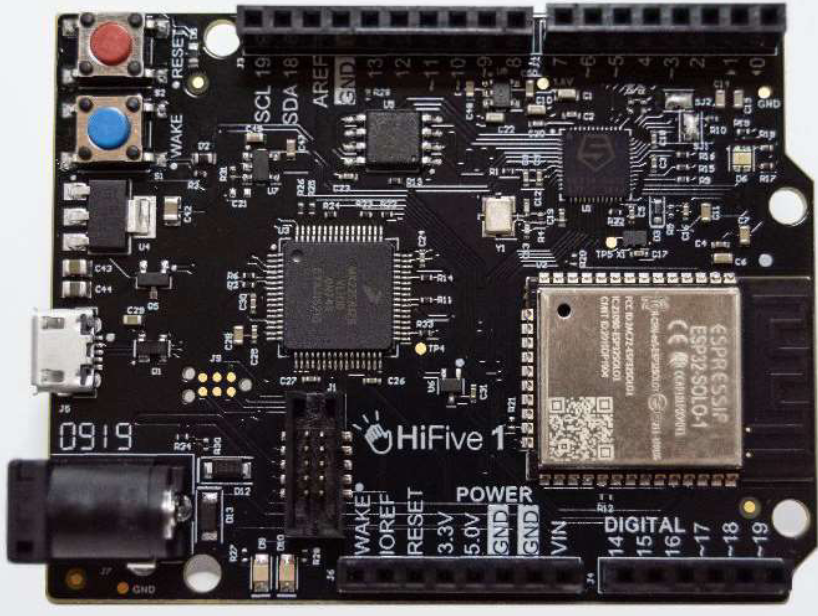
\includegraphics[width=0.6\columnwidth]{figures/board_image.png}
    \centering
    \caption[Sifive Hifive1 RevB]{This figure shows the Sifive Hifive1 RevB development board from the Hifive1 Rev B Schematics\cite{sifive_schematics}}
\end{figure}
This project will be done on the Sifive Hifive1 Rev B. This is the second iteration of the Hifive1 board, which uses the SiFive Freedom E310-G002 chip featuring a RV32IMAC core, a 16 KiB instruction cache, 16 KiB data RAM, and 512 Mib of flash memory, which acts as ROM. It has Arduino compatible pins, a set of LEDs, a Bluetooth/WiFi chip, and a USB interface.